\section{Implementation details}
Before applying the models, it was essential to prepare the data through standardization and splitting into training and testing sets. Standardization ensures that all features have a mean of 0 and a standard deviation of 1, making the data suitable for algorithms sensitive to feature scaling. This was achieved using the StandardScaler\cite{StandardScaler}:
\begin{python}
# Standardize
scaler = StandardScaler()
X = scaler.fit_transform(X)

# Split Data
X_train, X_test, y_train, y_test = 
        train_test_split(X, y, stratify=y, 
                    test_size=0.2, random_state=21)
\end{python}
The train-test split was performed with an 80-20 ratio, stratifying by the target variable to maintain class balance in both sets. This step ensures fair evaluation of the models on unseen data.

%\newline
%\bigskip
%\newline
%\bigskip
%\newline
%\bigskip\newline
%\bigskip
\subsection{Model Development Workflow}
For each of the \acrshort{ml} models applied in this study, the following sequence of steps was used:
\begin{enumerate}
\item Base Model:
The initial model was applied using default hyperparameters. This model serves as a baseline for comparison with subsequent models. By establishing baseline metrics such as Accuracy, F1 score, Precision, and Recall, we can evaluate the impact of further optimizations.

\item Hyperparameter Tuned Model:
To enhance the model’s performance, we focused on optimizing the hyperparameters, which balances regularization strength and data fitting. Using RandomizedSearchCV\cite{RandomizedSearchCV}:
\begin{python}
model = RandomizedSearchCV(
        hypertuned_model, 
        hyperparameters, 
        scoring="accuracy", 
        n_iter=n_iter, 
        random_state=42,  
        verbose=1
    )
\end{python}

\begin{itemize} \item Scoring Metric: Accuracy was used to evaluate the effectiveness of each parameter combination. \item Number of Iterations (n\_iter): Limited to ensure efficient exploration of the hyperparameter space. \end{itemize}

\item K-Fold Cross-Validation Model:
The optimized hyperparameter-tuned model was further evaluated using dynamic K-Fold Cross-Validation. Instead of fixing the number of folds at 5, the algorithm iteratively evaluated the model over k (in our case 10) folds, selecting the fold with the highest accuracy as the best estimator. This approach ensures that the model's performance generalizes well across different subsets of the data and identifies the optimal fold for the most reliable estimator.
\end{enumerate}

\section{Results}
\subsection{Logistic Regression}
We applied logistic regression using three approaches: the Base Model, the Hyper-Parameter Selection Model, and K-Fold Cross-Validation on the Hyper-Parameter Selection Model. 

\subsubsection{Base Model}
Table \ref{tab:tab1} presents the hyperparameters selected for the base model.

\begin{table}[ht]
    \centering
    \caption{Base hyperparameters in Logistic Regression} 
    \begin{tabular}{||c c c c c||} 
     \hline
     C & class\_weight & max\_iter & penalty & solver \\ [0.5ex] 
     \hline\hline
     1.0 & None & 100 & l2 & lbfgs \\ 
    \hline
    \end{tabular}
    \label{tab:tab1}
\end{table}

In the base Logistic Regression model, the following hyperparameters were used:

\begin{itemize}
    \item C: Set to 1.0, this hyperparameter controls the trade-off between model complexity and training accuracy. It is the inverse of the regularization strength. A smaller value increases regularization, reducing the influence of less important features, while a larger value prioritizes fitting the training data over regularization.
    \item class\_weight: Set to None, meaning no explicit balancing was applied to account for class imbalances.
    \item max\_iter: Defined as 100, this represents the maximum number of iterations the solver is allowed to perform to converge to a solution.
    \item penalty: The l2 regularization was used, which minimizes the sum of the squared coefficients to penalize large values and reduce overfitting.
    \item solver: The solver was set to lbfgs, an efficient optimization algorithm commonly used for logistic regression with small to medium-sized datasets.
\end{itemize}

The results for the Base Model application are:

\begin{figure}[H]
    \centering
    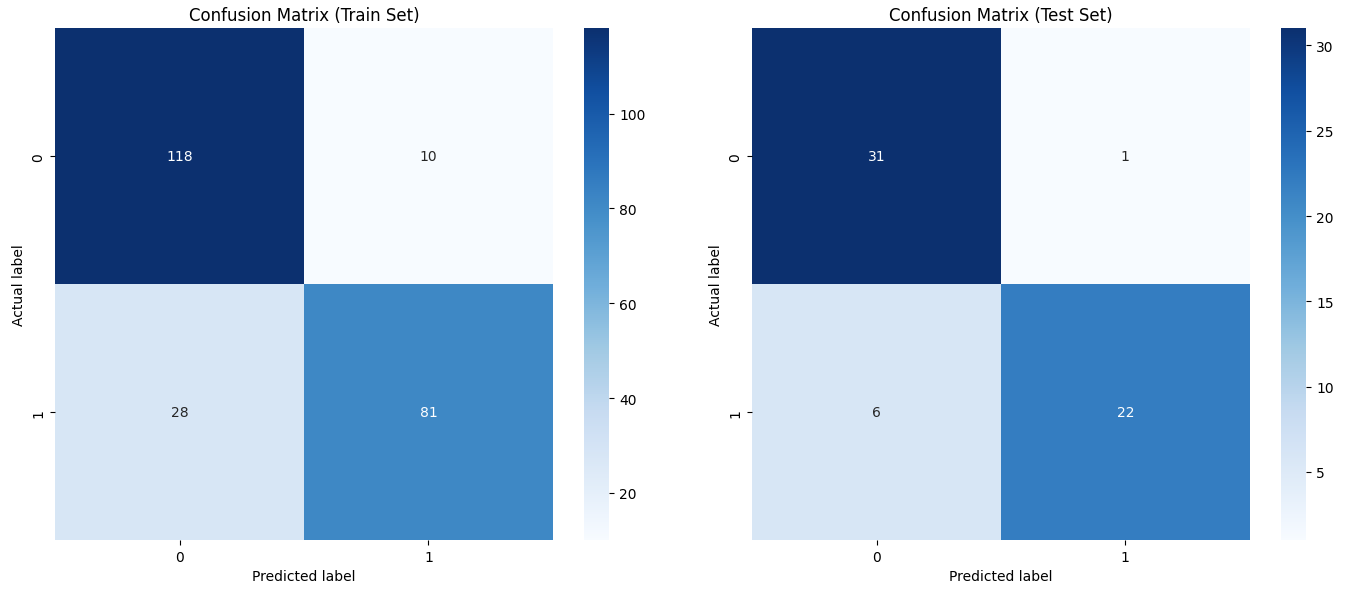
\includegraphics[width=1\linewidth]{images/confusion_matrix_lg_reg_base.png}
    \caption{Confusion Matrix}
    \label{fig:enter-label}
\end{figure}
\begin{figure}[H]
    \centering
    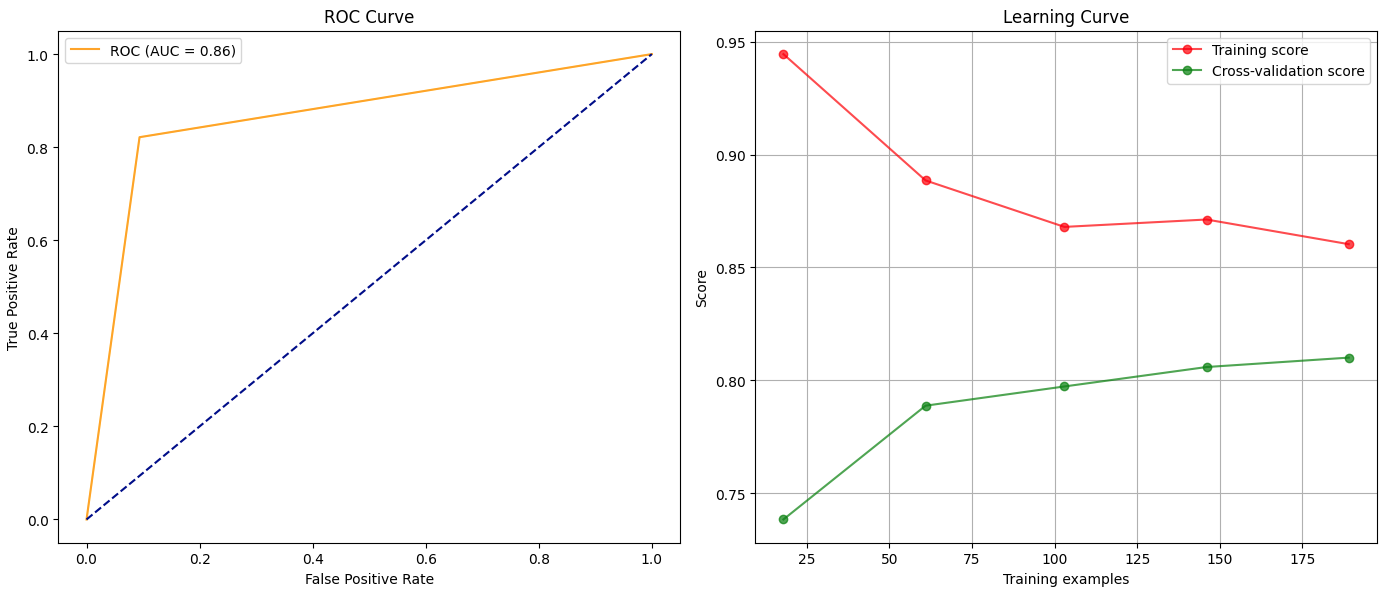
\includegraphics[width=1\linewidth]{images/roc_learning_logreg_base.png}
    \caption{ROC Curve and Learning Curve}%
    \label{fig:enter-label}
\end{figure}

\subsubsection{Hyper-Parameter Selection Model}

Next, we performed a search for the optimal value of C. The choice of C plays a critical role in determining the balance between fitting the training data and generalization. A value that is too small may lead to underfitting, while a very large value could lead to overfitting.

To find the best value for C, we employed RandomizedSearchCV with a range of values:
\begin{equation}
C \in \{0.001, 0.01, 0.1, 1, 10, 100\}
\end{equation}


\begin{table}[ht]
    \centering
    \caption{Best hyperparameters in Logistic Regression} 
    \begin{tabular}{||c c c c c||} 
     \hline
     C & class\_weight & max\_iter & penalty & solver \\ [0.5ex] 
     \hline\hline
     0.01 & None & 100 & l2 & lbfgs \\ 
    \hline
    \end{tabular}
    \label{tab:tab2}
\end{table}


The results for the Hyper-Parameter Selection Model are:
\begin{figure}[H]
    \centering
    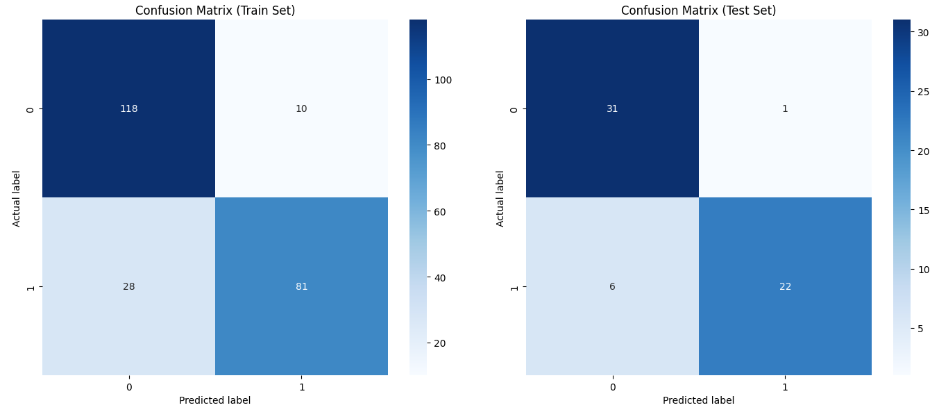
\includegraphics[width=1\linewidth]{images/confusion_matrix_lg_reg_search.png}
    \caption{Confusion Matrix}
    \label{fig:enter-label}
\end{figure}
\begin{figure}[H]
    \centering
    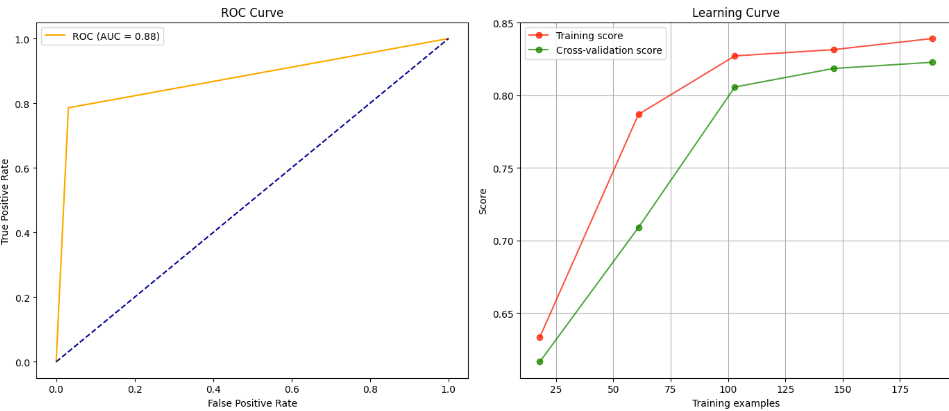
\includegraphics[width=1\linewidth]{images/roc_learning_logreg_search.png}
    \caption{ROC Curve and Learning Curve}%
    \label{fig:enter-label}
\end{figure}


\subsubsection{K-Fold Cross-Validation Model}

To evaluate the model's robustness and minimize the risk of overfitting, we applied K-Fold Cross-Validation. 

The results of the K-Fold Cross-Validation are shown in Figure \ref{fig:kfold_logReg}. Each fold's accuracy score is visualized, allowing us to identify the fold with the highest accuracy. In this case, the fold with the best performance was Fold 8, which achieved the highest accuracy.

\begin{figure}[H] \centering 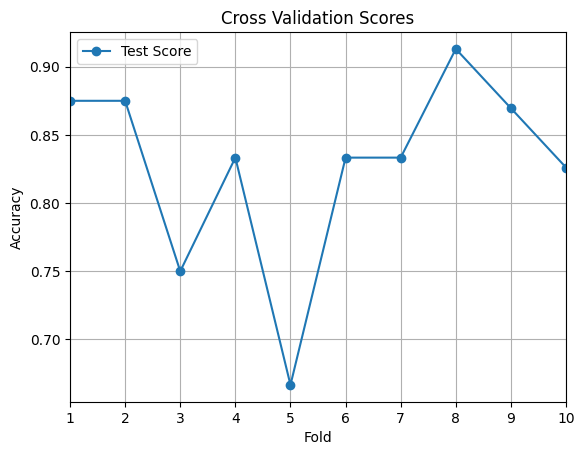
\includegraphics[width=0.75\linewidth]{images/k_fold_cross_log_reg.png} \caption{Accuracy Scores Across K-Folds} \label{fig:kfold_logReg} \end{figure}

Based on this result, the model corresponding to the best-performing fold (Fold 8) was selected and retrained on the entire training dataset. This ensures that the final model leverages all available training data while incorporating the insights gained from the cross-validation process.
The results for the K-Fold Cross-Validation Model are:

\begin{figure}[H]
    \centering
    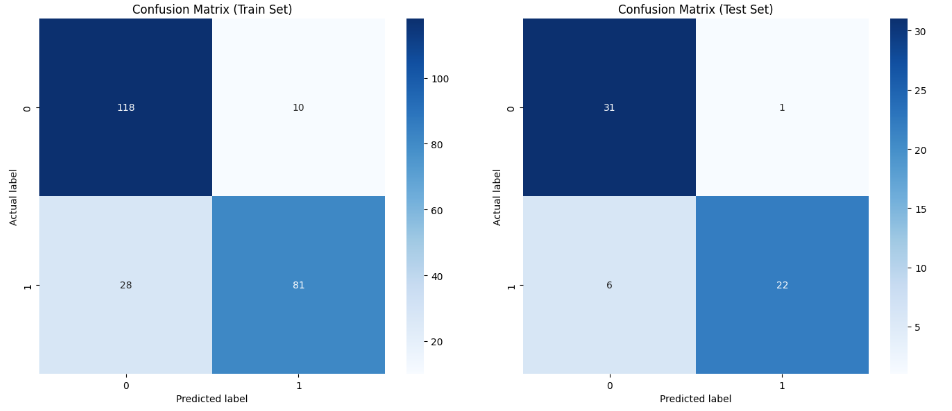
\includegraphics[width=1\linewidth]{images/confusion_matrix_lg_reg_kfold.png}
    \caption{Confusion Matrix}
    \label{fig:enter-label}
\end{figure}
\begin{figure}[H]
    \centering
    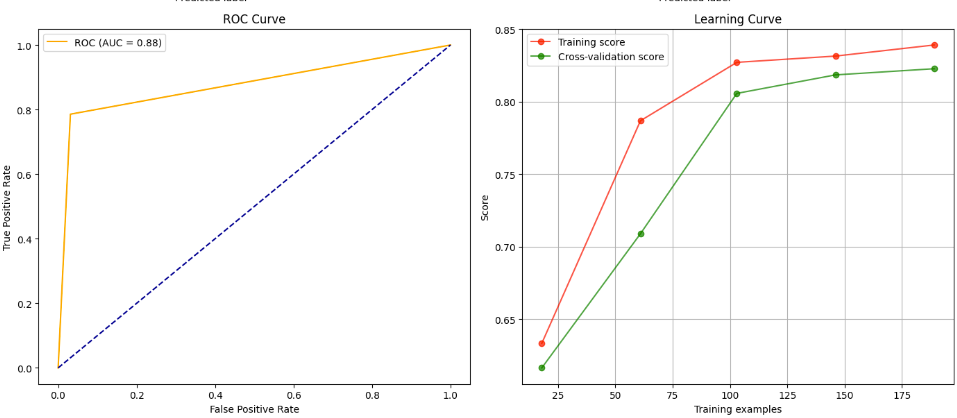
\includegraphics[width=1\linewidth]{images/roc_learning_logreg_kfold.png}
    \caption{ROC Curve and Learning Curve}%
    \label{fig:enter-label}
\end{figure}

\begin{figure}[H]
    \centering
    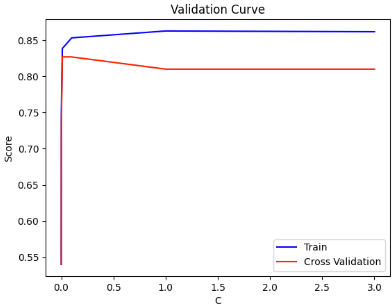
\includegraphics[width=0.75\linewidth]{images/validation_curve_log_reg.png}
    \caption{Validation Curve}
    \label{fig:ValidationCurveLogReg}
\end{figure}

\subsubsection{Conclusions}
Observing the confusion matrices, we can conclude that the number of incorrectly classified examples, the sum of \acrfull{FP} and \acrfull{FN}, is very low compared to the number of correctly classified examples, sum of \acrfull{TP} with \acrfull{TN}. Therefore, we can consider the model accurate.

The higher the AUC score, the better the performance of a classifier for a given task. Therefore, through the ROC Curve graphs, we can say that the classifier performed well because the AUC value is 0.86/0.88. It has good predictive power.

In Fig \ref{fig:ValidationCurveLogReg}, we observe that C values in the range between 0 and 3 are suitable, with the best performance concentrated in the interval from 0 to 2. After a value close to 0, both training accuracy and cross-validation accuracy stabilize, with training scores averaging around 0.85 and cross-validation scores around 0.81.

The differences between training and validation scores are minimal, indicating that the model achieves a good balance between bias and variance. This behavior suggests that variations in the C parameter within this range have an insignificant impact on the overall performance of the model, making it robust for this interval of values.

\begin{table}[H]
    \centering
    \caption{Classification - All Model} 
    \begin{tabular}{||c| c c c c||} 
     \hline
     & Accuracy & F1 Score & Recall & Precision \\
     \hline\hline
     Base Model & 0.867 & 0.852 & 0.821 & 0.885 \\
     \hline
    Hyper-Parameter & 0.883 & 0.863 & 0.79 & 0.957 \\ 
    \hline
    K-Fold & 0.883 & 0.863 & 0.79 & 0.957 \\ 
    \hline
    \end{tabular}
    \label{tab:tab_LogReg}
\end{table}

By examining Table \ref{tab:tab_LogReg}, we observe that the Accuracy and F1 Score for the Hyper-Parameter Selection Model and K-Fold Cross-Validation Model are identical, both slightly outperforming the Base Model. While the Base Model achieves a good Precision (0.885), the Hyper-Parameter and K-Fold models significantly improve it to 0.957, indicating a better ability to correctly identify true positive cases among all positive predictions.

However, the Recall (or Sensibility) is slightly lower for the Hyper-Parameter and K-Fold models (0.79) compared to the Base Model (0.821). This indicates that the Base Model is slightly better at identifying the real positive cases, but at the cost of reduced Precision.

In this context, even though it is critical to minimize false negatives because missing a cancer diagnosis can have more severe consequences than giving a false diagnosis, the Hyper-Parameter Selection and K-Fold models are preferable because they have a much higher Precision and their differences in Recall are minimal compared to the Base-Model.

%%%%%%%%%%%%%%%%%%%%%%%%%%%%%%%% SVC %%%%%%%%%%%%%%%%%%%%%%%%%
\bigskip
\subsection{Support Vector Machine}

We applied SVC using three approaches: the Base Model, the Hyper-Parameter Selection Model, and K-Fold Cross-Validation on the Hyper-Parameter Selection Model. 

\subsubsection{Base Model}
Table \ref{tab:tab1_svc} presents the parameters selected for the base model.

\begin{table}[ht]
    \centering
    \caption{Base parameters in SVC} 
    \begin{tabular}{||c c c c c||} 
     \hline
     C & class\_weight & max\_iter & gamma & kernel \\ [0.5ex] 
     \hline\hline
     1.0 & None & 100 & scale & rbf \\ 
    \hline
    \end{tabular}
    \label{tab:tab1_svc}
\end{table}

In the base SVC model, the following parameters were used:

\begin{itemize}
    \item C: Set to 1.0, this hyperparameter controls the trade-off between model complexity and training accuracy. It is the inverse of the regularization strength. A smaller value increases regularization, reducing the influence of less important features, while a larger value prioritizes fitting the training data over regularization.
    \item class\_weight: Set to None, meaning no explicit class balancing was applied. This can lead to biased results in imbalanced datasets. 
    \item max\_iter: Defined as 100, representing the maximum number of iterations the solver is allowed to perform to reach convergence. If the solver does not converge within 100 iterations, the process stops. 
    \item gamma: Set to "scale," which automatically calculates the gamma parameter as \[
    \gamma = \frac{1}{\text{number of features}}
    \] This controls the influence of a single training example, with higher values leading to tighter decision boundaries.
    \item kernel: Set to rbf (Radial Basis Function), which is a popular kernel function in SVC models. It allows the model to capture non-linear relationships between features by mapping the data into a higher-dimensional space.
\end{itemize}

The results for the Base Model application are:

\begin{figure}[H]
    \centering
    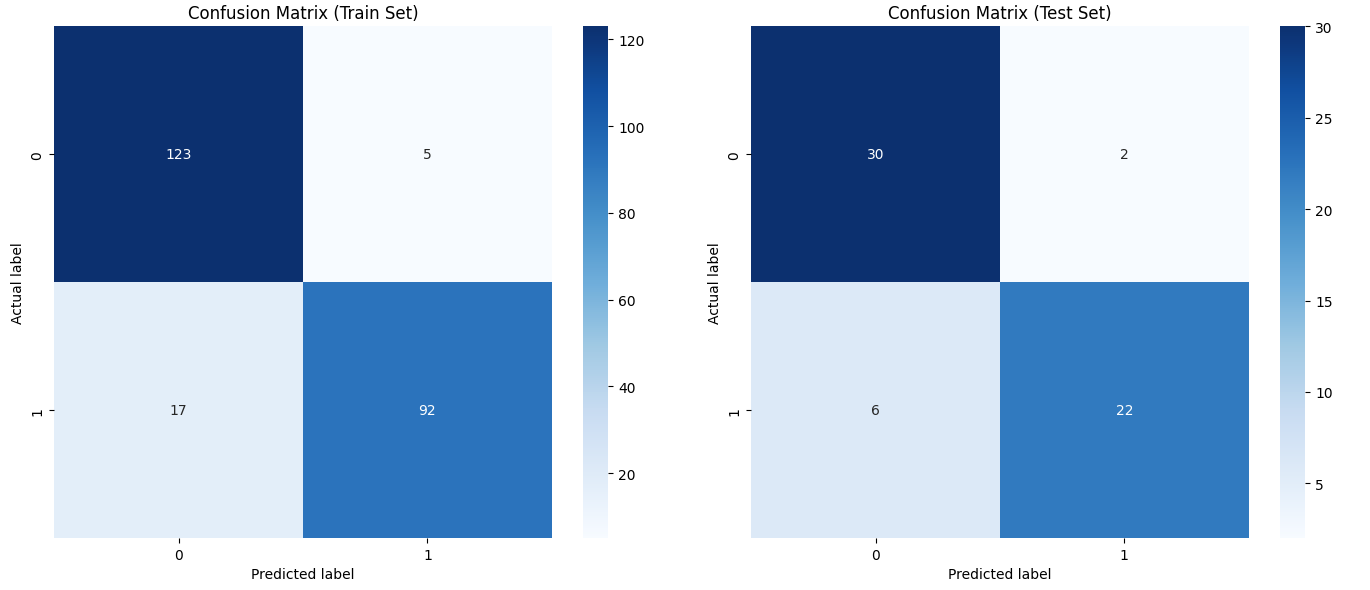
\includegraphics[width=1\linewidth]{images/confusion_matrix_svc_base.png}
    \caption{Confusion Matrix}
    \label{fig:enter-label}
\end{figure}
\begin{figure}[H]
    \centering
    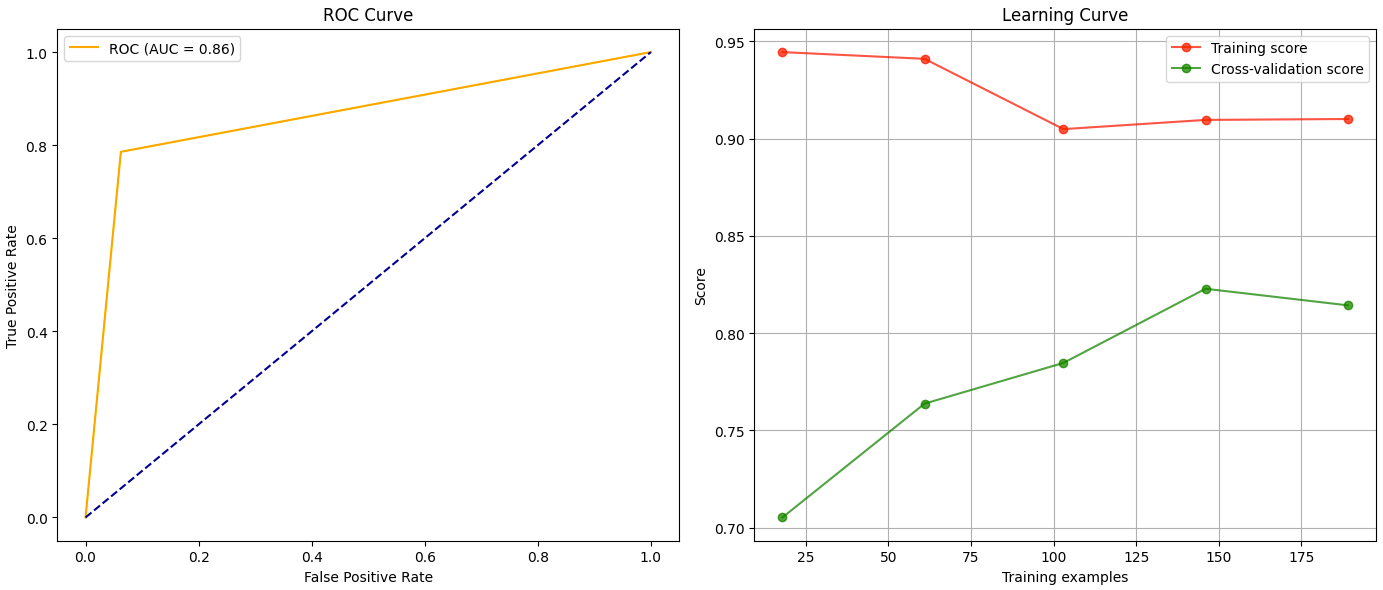
\includegraphics[width=1\linewidth]{images/roc_learning_svc_base.png}
    \caption{ROC Curve and Learning Curve}%
    \label{fig:enter-label}
\end{figure}

\subsubsection{Hyper-Parameter Selection Model}

Next, we performed a search for the optimal values of C, the regularization parameter, and gamma, the kernel coefficient. Both parameters play a critical role in determining the model's performance.

\begin{itemize}
    \item \textbf{C} controls the trade-off between fitting the training data and applying regularization. A smaller value of C increases regularization, which can lead to underfitting, while a larger value reduces regularization, potentially leading to overfitting.
    \item \textbf{gamma} defines how far the influence of a single training example reaches. Higher values of gamma result in tighter decision boundaries, which can capture more complex patterns but may also lead to overfitting. Lower values lead to smoother decision boundaries and better generalization.
    \item \textbf{kernel}: The kernel function is used to map the original data into a higher-dimensional space, where a linear decision boundary can separate the data more effectively. We experimented with different kernel functions:
\begin{itemize}
    \item rbf (Radial Basis Function): This is the most commonly used kernel, which computes the similarity between points using the distance between them, allowing for non-linear decision boundaries.
    \item linear: This kernel is used when the data is linearly separable, and it directly applies a linear decision boundary.
    \item poly (Polynomial): This kernel allows for decision boundaries based on polynomial functions of the input features, making it suitable for datasets with more complex, but still polynomially separable, relationships.
\end{itemize}
\end{itemize}

To find the optimal values for these parameters, we employed RandomizedSearchCV with the following ranges:
\begin{equation}
C \in \{0.01, 0.1, 1, 10, 100\}
\end{equation}
\begin{equation}
gamma \in \{10, 1, 0.1, 0.01, 0.001\}
\end{equation}
\begin{equation}
kernel \in \{'rbf','linear','poly'\}
\end{equation}


\begin{table}[ht]
    \centering
    \caption{Best parameters in SVC} 
    \begin{tabular}{||c c c c c||} 
     \hline
     C & class\_weight & max\_iter & gamma & kernel \\ [0.5ex] 
     \hline\hline
     0.01 & None & 100 & 1 & linear\\ 
    \hline
    \end{tabular}
    \label{tab:tab2_svc}
\end{table}

The results for the Hyper-Parameter Selection Model are:
\begin{figure}[H]
    \centering
    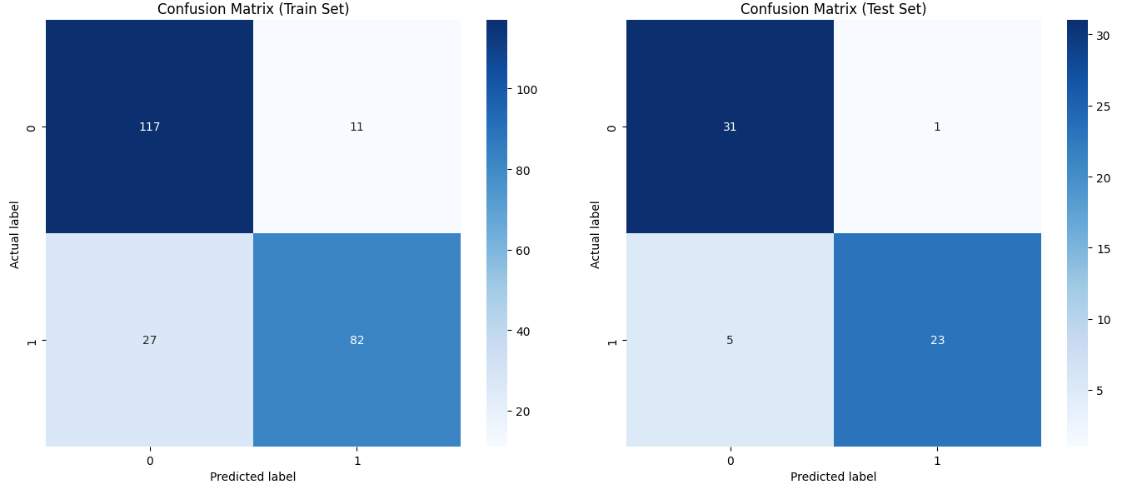
\includegraphics[width=1\linewidth]{images/confusion_matrix_svc_search.png}
    \caption{Confusion Matrix}
    \label{fig:enter-label}
\end{figure}
\begin{figure}[H]
    \centering
    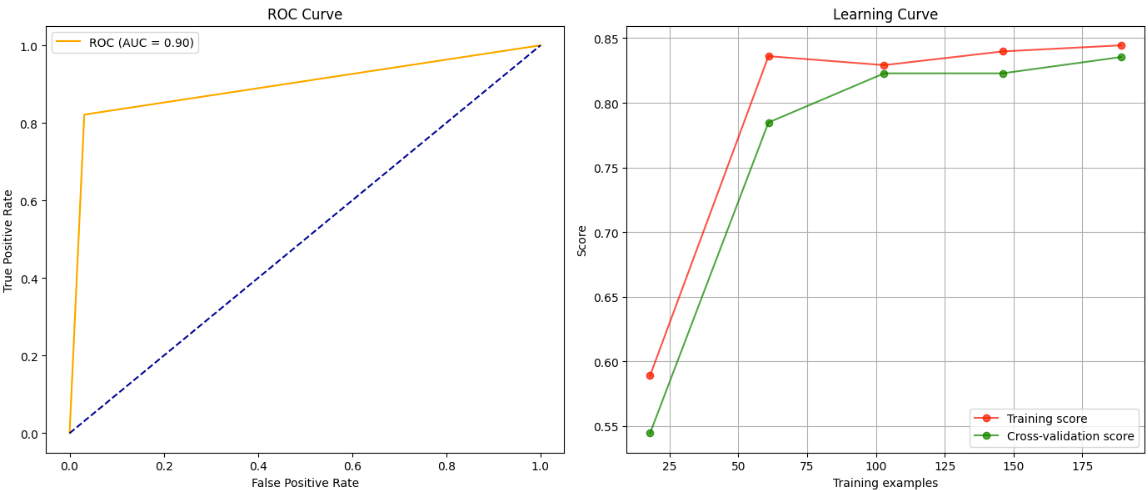
\includegraphics[width=1\linewidth]{images/roc_learning_svc_search.png}
    \caption{ROC Curve and Learning Curve}%
    \label{fig:enter-label}
\end{figure}


\subsubsection{K-Fold Cross-Validation Model}

To evaluate the model's robustness and minimize the risk of overfitting, we applied K-Fold Cross-Validation. 

The results of the K-Fold Cross-Validation are shown in Figure \ref{fig:k_fold_cross_svc.png}. Each fold's accuracy score is visualized, allowing us to identify the fold with the highest accuracy. In this case, the fold with the best performance was Fold 2, which achieved the highest accuracy.

\begin{figure}[H] \centering 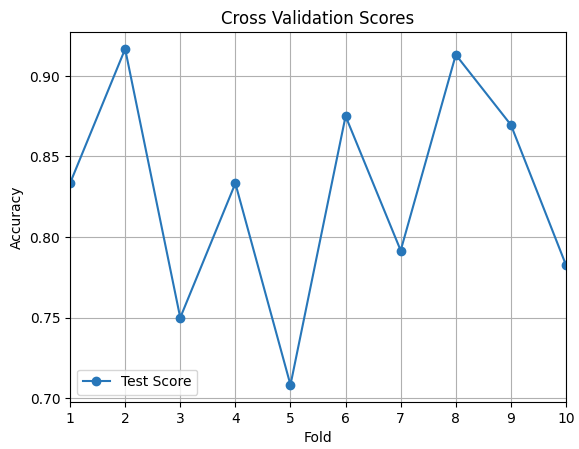
\includegraphics[width=0.75\linewidth]{images/k_fold_cross_svc.png} \caption{Accuracy Scores Across K-Folds} \label{fig:k_fold_cross_svc.png} \end{figure}

Based on this result, the model corresponding to the best-performing fold (Fold 2) was selected and retrained on the entire training dataset. This ensures that the final model leverages all available training data while incorporating the insights gained from the cross-validation process.

The results for the K-Fold Cross-Validation Model are:

\begin{figure}[H]
    \centering
    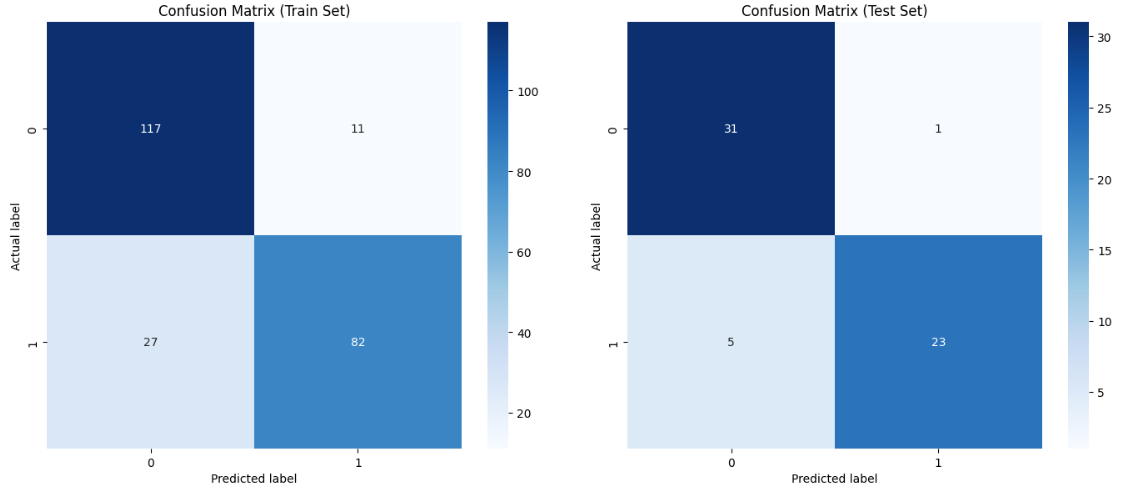
\includegraphics[width=1\linewidth]{images/confusion_matrix_svc_kfold.png}
    \caption{Confusion Matrix}
    \label{fig:enter-label}
\end{figure}
\begin{figure}[H]
    \centering
    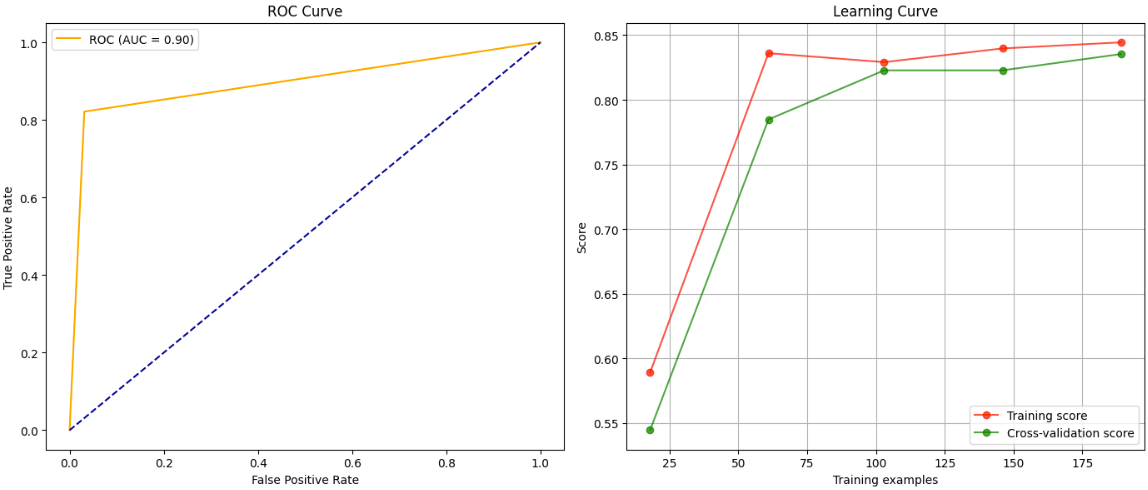
\includegraphics[width=1\linewidth]{images/roc_learning_svc_kfold.png}
    \caption{ROC Curve and Learning Curve}%
    \label{fig:enter-label}
\end{figure}

\begin{figure}[H]
    \centering
    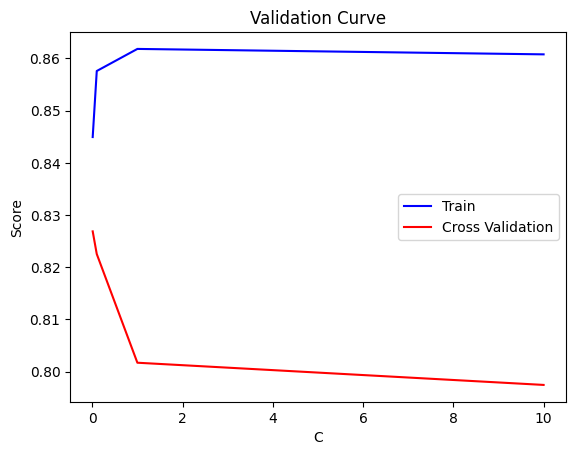
\includegraphics[width=0.75\linewidth]{images/validation_curve_c_svc.png}
    \caption{Validation Curve}
    \label{fig:ValidationCurveC_SVC}
\end{figure}
\begin{figure}[H]
    \centering
    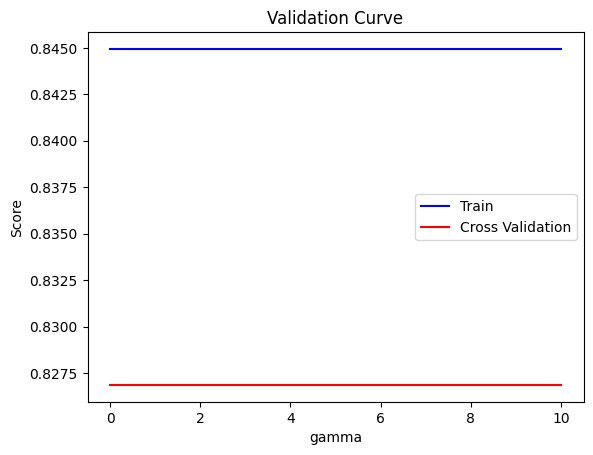
\includegraphics[width=0.75\linewidth]{images/validation_curve_gamma_svc.png}
    \caption{Validation Curve}
    \label{fig:ValidationCurveGamma_SVC}
\end{figure}

\subsubsection{Conclusions}
As observed previously in the Logistic Regression results, the confusion matrices for the Support Vector Classifier (SVC) also show that the number of incorrectly classified examples, the sum of \acrfull{FP} and \acrfull{FN}, is very low compared to the number of correctly classified examples, the sum of \acrfull{TP} and \acrfull{TN}. Therefore, we can conclude that the model demonstrates high accuracy, similar to the Logistic Regression model.

In addition, the AUC values for the SVC, as with the Logistic Regression, range between 0.86 and 0.90, indicating consistent and strong predictive power across both classifiers.

In Fig. \ref{fig:ValidationCurveC_SVC} (C), we observe that C values in the range between 0 and 3 are suitable, with the best performance concentrated in the interval from 0 to 2. Beyond a value close to 0, both training accuracy and cross-validation accuracy stabilize, with training scores averaging around 0.86 and cross-validation scores around 0.81. This stability suggests that variations in the C parameter within this range have minimal impact on the model's performance, making it robust and well-balanced between bias and variance.

In Fig. \ref{fig:ValidationCurveGamma_SVC} (gamma), we observe that the value of gamma does not require adjustments when using the linear kernel. Since the kernel is linear, the gamma parameter does not affect the model’s performance, and no significant changes are observed.

Thus, as with Logistic Regression, selecting moderate values for C ensures a better balance between bias and variance, leading to a more generalizable and robust SVC model.

\begin{table}[H]
    \centering
    \caption{Classification - All Model} 
    \begin{tabular}{||c| c c c c||} 
     \hline
     & Accuracy & F1 Score & Recall & Precision \\
     \hline\hline
     Base Model & 0.867 & 0.846 & 0.786 & 0.917 \\
     \hline
    Hyper-Parameter & 0.900 & 0.885 & 0.821 & 0.958 \\ 
    \hline
    K-Fold & 0.900 & 0.885 & 0.821 & 0.958 \\ 
    \hline
    \end{tabular}
    \label{tab:tab_SvcFinal}
\end{table}

By examining Table \ref{tab:tab_SvcFinal}, we observe that the Accuracy and F1 Score for the Hyper-Parameter Selection Model and K-Fold Cross-Validation Model are identical, both slightly outperforming the Base Model. While the Base Model achieves a good Precision of 0.917, the Hyper-Parameter and K-Fold models significantly improve it to 0.958, indicating a better ability to correctly identify true positive cases among all positive predictions.

However, the Recall (or Sensibility) is identical for both the Hyper-Parameter and K-Fold models (0.821) and slightly lower than the Base Model (0.786), suggesting that all models perform similarly in identifying actual positive cases. The Base Model has a slight edge in this regard, but the difference is minimal.

In this context, even though it is critical to minimize false negatives because missing a cancer diagnosis can have more severe consequences than giving a false diagnosis, the Hyper-Parameter Selection and K-Fold models are preferable because they have better overall higher values in their metrics and the differences in Recall are minimal compared to the Base-Model.

%%%%%%%%%%%%%%%%%%%%%%%%%%%%%%%% Neural Network %%%%%%%%%%%%%%%%%%%%%%%%%
\bigskip
\subsection{Neural Network}

We applied Multilayer Perceptron using three approaches: the Base Model, the Hyper-Parameter Selection Model, and K-Fold Cross-Validation on the Hyper-Parameter Selection Model. 

\subsubsection{Base Model}
Table \ref{tab:tab1_mlp} presents the parameters selected for the base model.

\begin{table}[ht]
    \centering
    \caption{Base parameters in MLP} 
    \begin{tabular}{||c c c c||} 
     \hline
     alpha & hidden\_layer\_sizes & learning\_rate & max\_iter  \\ [0.5ex] 
     \hline\hline
     0.0001 & (100,) & constant & 200 \\ 
    \hline
    \end{tabular}
    \label{tab:tab1_mlp}
\end{table}

In the base MLP model, the following parameters were used:

\begin{itemize}
\item alpha: Set to 0.0001, this parameter controls the strength of the regularization. It helps to prevent overfitting by penalizing large weights in the model. A smaller value allows the model to fit the training data more closely, while a larger value increases regularization, simplifying the model.

\item hidden\_layer\_sizes: Set to (100,), meaning the model uses a single hidden layer with 100 neurons. This configuration determines the complexity of the model, as more neurons can capture more complex patterns in the data.

\item learning\_rate: Set to constant, which means the learning rate remains constant throughout the training process. A constant learning rate helps maintain stable training behavior but may require careful tuning to achieve optimal results.

\item max\_iter: Defined as 200, this parameter represents the maximum number of iterations the solver is allowed to perform to converge. If the solver does not converge within 200 iterations, the training process is stopped. This ensures that the model doesn't train indefinitely if convergence is not reached.

\end{itemize}

The results for the Base Model application are:

\begin{figure}[H]
    \centering
    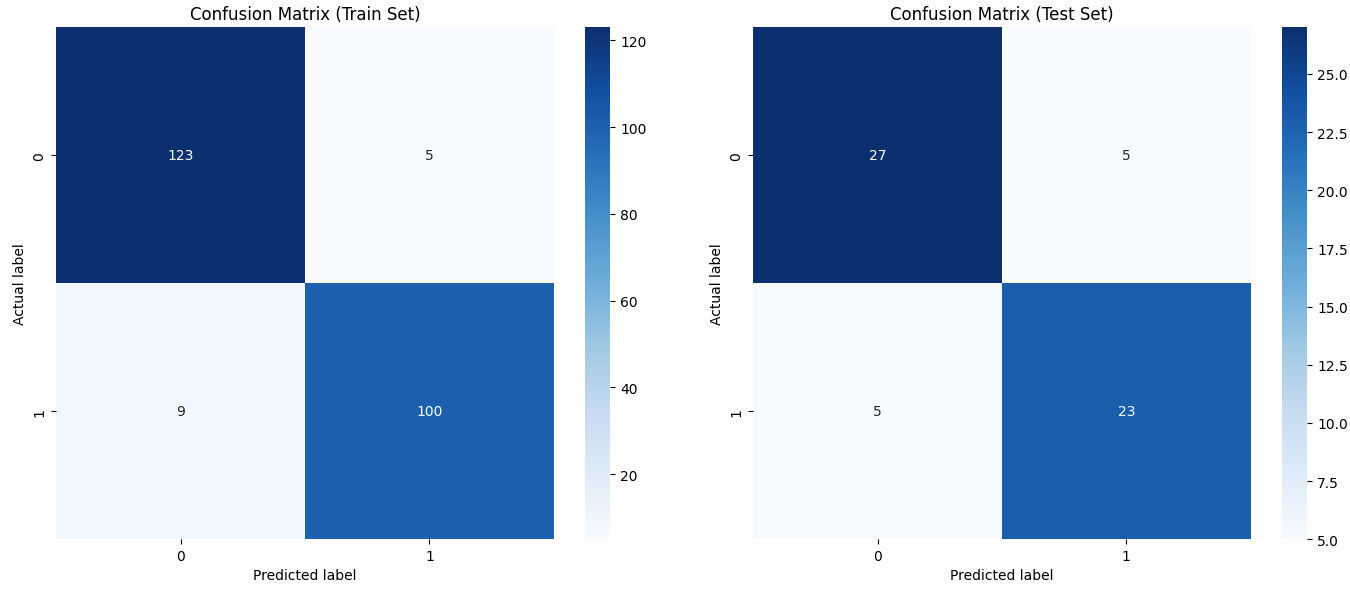
\includegraphics[width=1\linewidth]{images/confusion_matrix_mlp_base.png}
    \caption{Confusion Matrix}
    \label{fig:enter-label}
\end{figure}
\begin{figure}[H]
    \centering
    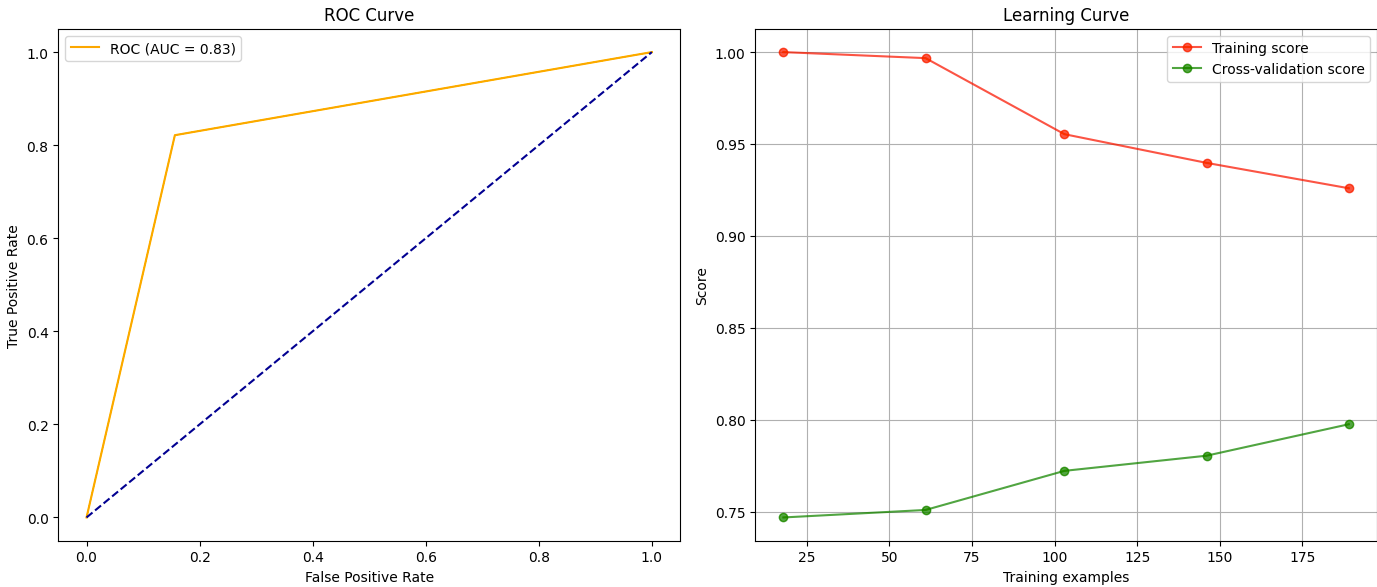
\includegraphics[width=1\linewidth]{images/roc_learning_mlp_base.png}
    \caption{ROC Curve and Learning Curve}%
    \label{fig:enter-label}
\end{figure}

\subsubsection{Hyper-Parameter Selection Model}

Next, we performed a search for the optimal values of the learning rate, alpha, and hidden layer sizes. These parameters play a critical role in determining the performance of the Multilayer Perceptron (MLP) model.

\begin{itemize} 
    \item \textbf{learning\_rate\_init}: Controls the initial step size for the gradient descent optimization process. Smaller values result in a slower, more stable convergence, while larger values speed up convergence but may cause instability or overshooting. 
    \item \textbf{alpha}: The regularization parameter, which controls the strength of L2 regularization. Higher values increase regularization and prevent overfitting, while smaller values allow the model to fit the training data more closely, potentially leading to overfitting. 
    
    \item \textbf{hidden\_layer\_sizes}: Specifies the number and size of hidden layers in the neural network. Larger networks with more neurons can capture more complex patterns but may also lead to overfitting. 
\end{itemize}

To find the optimal values for these parameters, we employed RandomizedSearchCV with the following ranges:

\begin{equation} learning\_rate\_init \in {0.001, 0.005, 0.01, 0.02} \end{equation} \begin{equation} alpha \in {0.0001, 0.001, 0.01} \end{equation} 
\begin{equation} hidden\_layer\_sizes \in {(10), (25), (50), (100), (10, 10), (20, 20)} \end{equation}

By using RandomizedSearchCV, we were able to efficiently explore the possible combinations of these hyperparameters and identify the best configuration for maximizing the model's performance.

\begin{table}[ht]
    \centering
    \caption{Best parameters in MLP} 
    \begin{tabular}{||c c c c||} 
     \hline
     alpha & hidden\_layer\_sizes & learning\_rate & max\_iter  \\ [0.5ex] 
     \hline\hline
     0.001 & (25,) & 0.001 & 200 \\ 
    \hline
    \end{tabular}
    \label{tab:tab2_mlp}
\end{table}

The results for the Hyper-Parameter Selection Model are:
\begin{figure}[H]
    \centering
    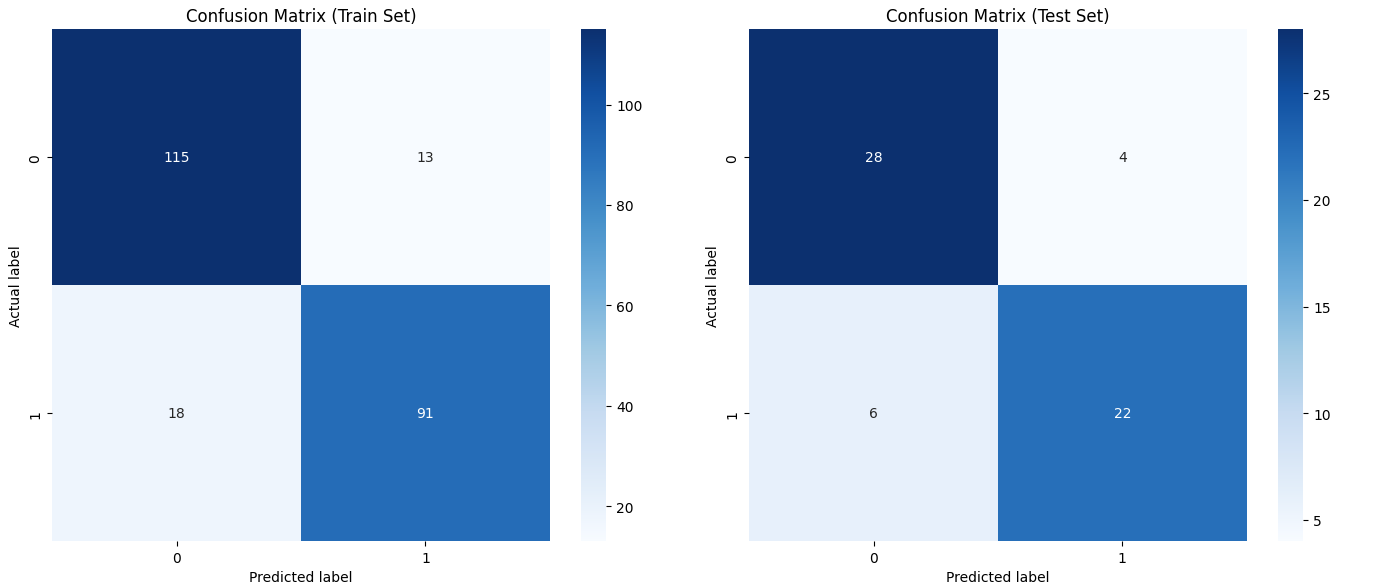
\includegraphics[width=1\linewidth]{images/confusion_matrix_mlp_search.png}
    \caption{Confusion Matrix}
    \label{fig:enter-label}
\end{figure}
\begin{figure}[H]
    \centering
    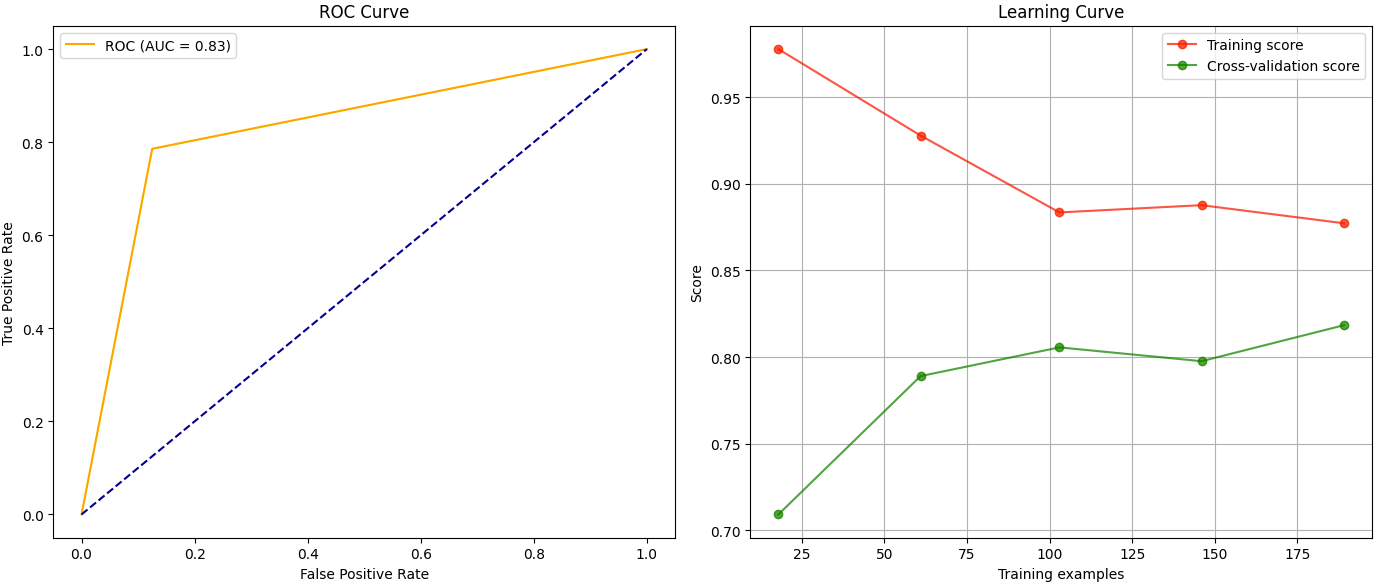
\includegraphics[width=1\linewidth]{images/roc_learning_mlp_search.png}
    \caption{ROC Curve and Learning Curve}%
    \label{fig:enter-label}
\end{figure}


\subsubsection{K-Fold Cross-Validation Model}

To evaluate the model's robustness and minimize the risk of overfitting, we applied K-Fold Cross-Validation. 

The results of the K-Fold Cross-Validation are shown in Figure \ref{fig:k_fold_cross_mlp.png}. Each fold's accuracy score is visualized, allowing us to identify the fold with the highest accuracy. In this case, the fold with the best performance was Fold 8, which achieved the highest accuracy.

\begin{figure}[H] \centering 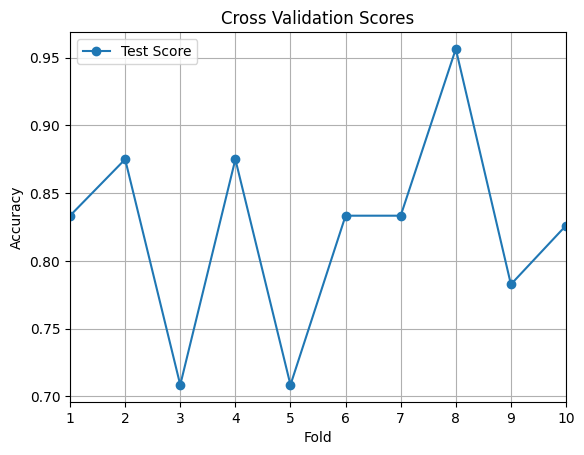
\includegraphics[width=0.75\linewidth]{images/k_fold_cross_mlp.png} \caption{Accuracy Scores Across K-Folds} \label{fig:k_fold_cross_svc.png} \end{figure}

Based on this result, the model corresponding to the best-performing fold (Fold 8) was selected and retrained on the entire training dataset. This ensures that the final model leverages all available training data while incorporating the insights gained from the cross-validation process.

The results for the K-Fold Cross-Validation Model are:

\begin{figure}[H]
    \centering
    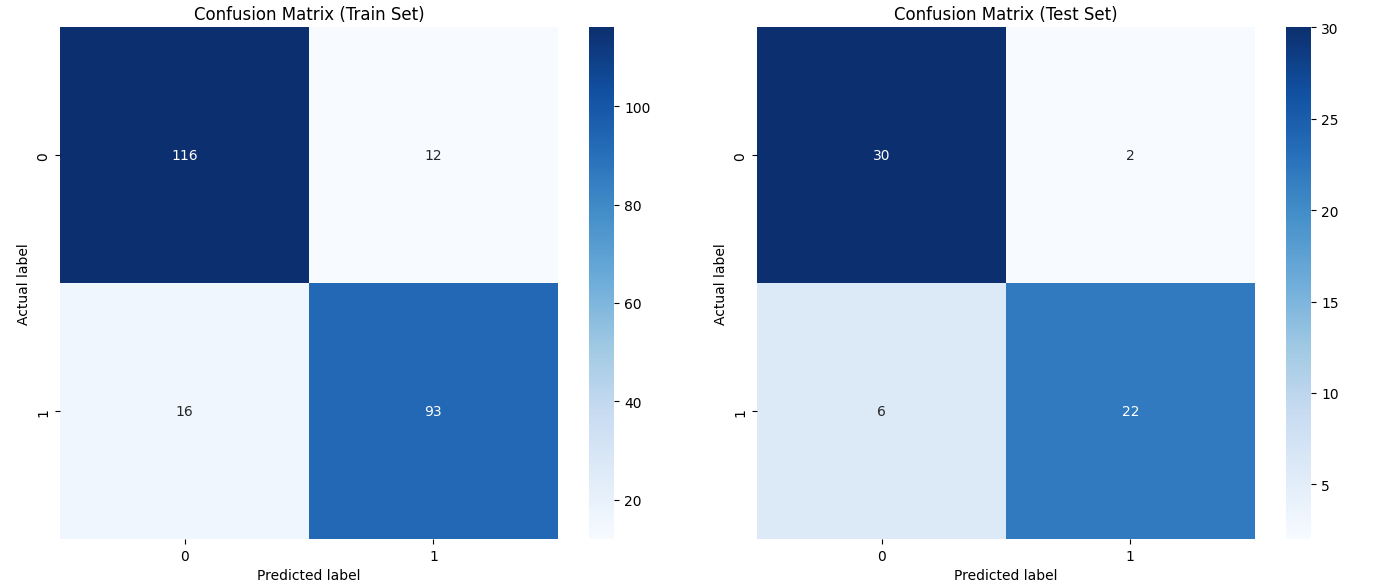
\includegraphics[width=1\linewidth]{images/confusion_matrix_mlp_kfold.png}
    \caption{Confusion Matrix}
    \label{fig:enter-label}
\end{figure}
\begin{figure}[H]
    \centering
    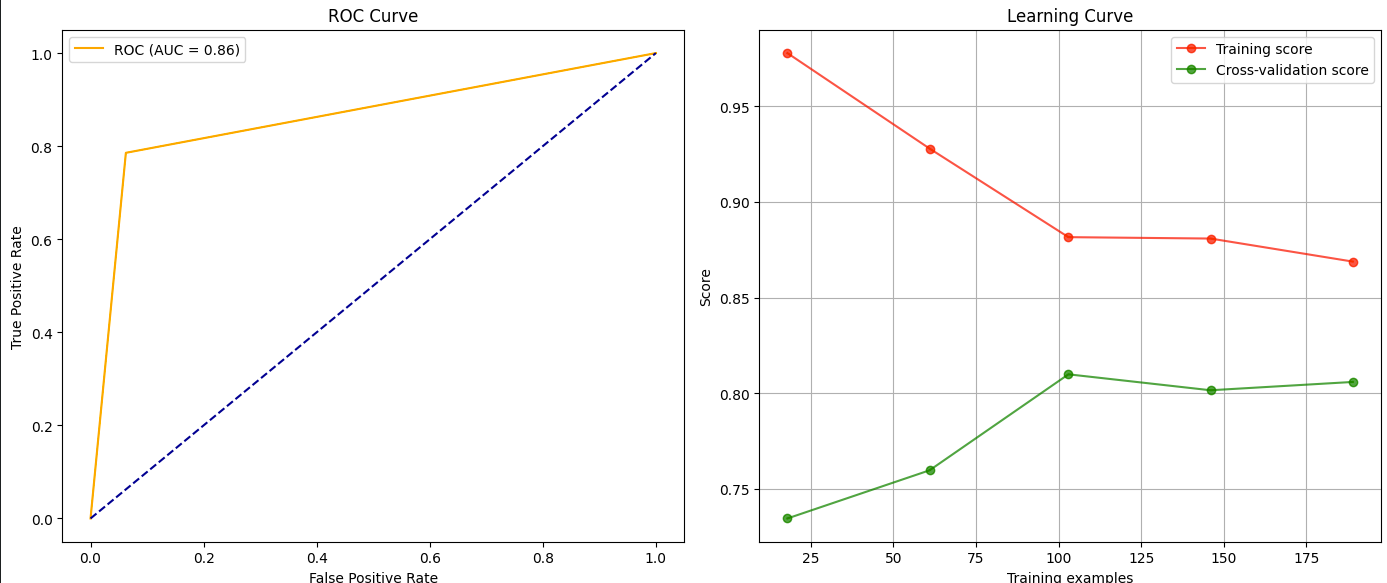
\includegraphics[width=1\linewidth]{images/roc_learning_mlp_kfold.png}
    \caption{ROC Curve and Learning Curve}%
    \label{fig:enter-label}
\end{figure}

\begin{figure}[H]
    \centering
    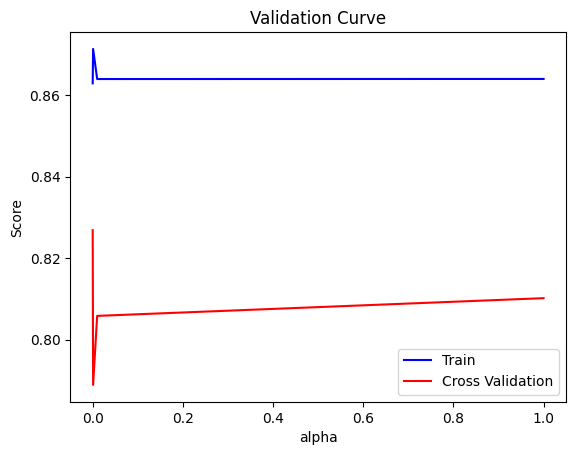
\includegraphics[width=0.75\linewidth]{images/ValidationCurveMLP_alpha.png}
    \caption{Validation Curve}
    \label{fig:ValidationCurveMLP_alpha}
\end{figure}
\begin{figure}[H]
    \centering
    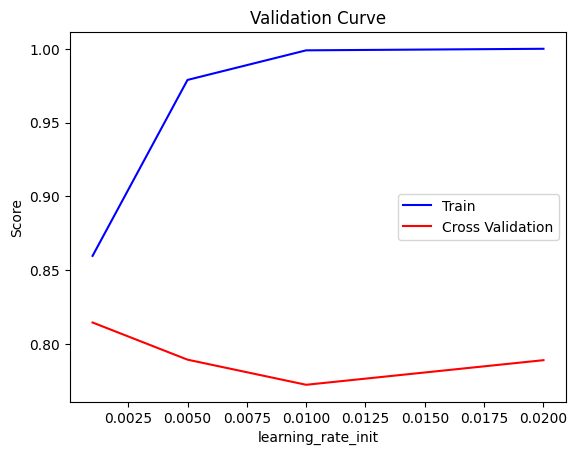
\includegraphics[width=0.75\linewidth]{images/ValidationCurveMLP_learning.png}
    \caption{Validation Curve}
    \label{fig:ValidationCurveGamma_SVC}
\end{figure}

\subsubsection{Conclusions}
As observed previously in the results, the confusion matrices show that the number of incorrectly classified examples, the sum of FP and FN, is very low compared to the number of correctly classified examples, the sum of TP and TN. This reinforces the model's accuracy and predictive power.

In addition, the AUC values for the MLP are slightly lower than those of other models, ranging between 0.83 and 0.86, but still indicating consistent and strong predictive power across both classifiers.

In Fig. \ref{fig:ValidationCurveMLP_alpha Curve}, we observe that alpha values in the range between 0 and 1 are suitable, with the best performance concentrated in the interval from 0 to 0.1. After a value close to 0, both training accuracy and cross-validation accuracy stabilize, with training scores around 0.86 and cross-validation scores around 0.80. This suggests that alpha values within this range provide a good balance between regularization and model fitting, ensuring that the model is neither too simple (underfitting) nor too complex (overfitting).

In the second graph, the analysis of the learning rate (learning\_rate\_init) shows that values between 0.0025 and 0.01 offer a good balance between training accuracy and cross-validation accuracy. Training scores reach up to 1.00, while cross-validation scores stabilize around 0.85, indicating that the model has learned well from the data without overfitting.

\begin{table}[H]
    \centering
    \caption{Classification - All Model} 
    \begin{tabular}{||c| c c c c||} 
     \hline
     & Accuracy & F1 Score & Recall & Precision \\
     \hline\hline
     Base Model & 0.833 & 0.821 & 0.821 & 0.821 \\
     \hline
    Hyper-Parameter & 0.833 & 0.815 & 0.786 & 0.846 \\ 
    \hline
    K-Fold & 0.868 & 0.846 & 0.786 & 0.917 \\ 
    \hline
    \end{tabular}
    \label{tab:tab_MLPFinal}
\end{table}

By examining Table \ref{tab:tab_MLPFinal}, we observe that the Accuracy and F1 Score for the Hyper-Parameter Selection Model and K-Fold Cross-Validation Model are identical, both slightly outperforming the Base Model. While the Base Model achieves a good Precision of 0.821, the Hyper-Parameter and K-Fold models improve this to 0.846 and 0.917, respectively. This indicates that the K-Fold model is the most effective at correctly identifying true positive cases among all positive predictions.

However, the Recall (or True Positive Rate) is slightly lower for the Hyper-Parameter and K-Fold models (0.786) compared to the Base Model (0.821), meaning the Base Model is marginally better at identifying actual positive cases, but at the cost of lower Precision.

The K-Fold model is the most preferable one because it has the highest values in all performance metrics except for recall where the differences are minimal in comparison with the other models.

\bigskip
\subsection{Comparison between the models}
The comparison between the models is based on the following performance metrics: Accuracy, F1 Score, Recall, and Precision. These metrics allow us to assess how well the models perform in terms of both correctly classifying positive and negative cases and minimizing false positives and false negatives.
\begin{itemize}
    \item \textbf{Accuracy} measures the overall correctness of the model by calculating the ratio of correct predictions to the total number of predictions.
    \item \textbf{F1 Score} is the harmonic mean of Precision and Recall, providing a balance between the two, especially when dealing with imbalanced classes.
    \item \textbf{Recall} (or True Positive Rate) measures the ability of the model to correctly identify positive instances.
    \item \textbf{Precision} measures the accuracy of positive predictions made by the model.
\end{itemize}

All models presented here underwent hyperparameter tuning using RandomizedSearchCV to find the optimal settings for each model. Additionally, K-Fold Cross-Validation was applied to ensure the robustness and generalizability of the results, providing a reliable estimate of how the models would perform on unseen data.

Below is the comparison table of the three models:

\begin{table}[H]
    \centering
    \caption{Comparison - All Model} 
    \begin{tabular}{||c| c c c c||} 
     \hline
     & Accuracy & F1 Score & Recall & Precision \\
     \hline\hline
     LR & 0.883 & 0.863 & 0.786 & 0.957 \\ 
     \hline
    SVC & 0.900 & 0.885 & 0.821 & 0.958  \\
    \hline
    MLP & 0.868 & 0.846 & 0.786 & 0.917 \\ 
    \hline
    \end{tabular}
    \label{tab:tab_Final}
\end{table}

Based on the results in Table \ref{tab:tab_Final}, we can observe the following:

\begin{itemize}
     \item The Logistic Regression (LR) model has an Accuracy of 0.883, an F1 Score of 0.863, and a Precision of 0.957. These results indicate that LR is effective at identifying true positive cases while maintaining a low rate of false positives.
    \item The Support Vector Classifier (SVC) model shows a higher Accuracy (0.900) and F1 Score (0.885) compared to the LR model, with Precision still being high (0.958). This suggests that SVC outperforms LR in terms of overall accuracy and balance between Precision and Recall.
    
    \item The MLP (Multilayer Perceptron), while having a lower Accuracy (0.868) and F1 Score (0.8463), still demonstrates good Precision (0.917). However, its overall performance is not as strong as SVC or LR.

\end{itemize}

The slightly lower performance of the MLP model can be attributed to several factors. One key reason could be the limited amount of training data available, which may not be sufficient to fully leverage the complexity of neural networks like MLP. Neural networks generally require large datasets to train effectively and avoid overfitting. Without enough data, the MLP model may not generalize well, which could explain its slightly lower performance compared to the SVC and LR models.

In this context, the SVC model emerges as the best performer, with the highest Accuracy and F1 Score, closely followed by LR. Both models show excellent Precision, making them suitable for applications where false positives must be minimized.